\subsection {Datenstruktur für Strecken / Geraden}
Zentral für die Lösungsidee ist eine effiziente Berechnung von Schnittpunkten
zwischen den Strecken.
Wie beschrieben werden dafür die Strecken in Geraden konvertiert.

Zu jeder möglichen Kombination aus zwei Punkten lässt sich wie beschrieben
entweder eine Gerade mit einer Funktionsgleichung vom Typen \(y=mx+n\) oder
eine Senkrechte parallel zur y-Achse mit einer Funktionsgleichung vom Typen \(x=n\)
bilden.
Bei letzterer entspricht  \(n\) dann logischerweise der gemeinsamen x-Koordinate.

Wenn eine lineare Funktion vom Typen \(y=mx+n\) aufgestellt wird,
kann deren Steigung \(m\) mit folgender Rechnung ermittelt werden:
\begin{equation}
    m=\frac{y_{P2} - y_{P1}}{x_{P2} - x_{P1}}
\end{equation}

Der y-Achsenabschnitt \(n\) ergibt sich aus folgender Rechnung:
\begin{equation}
    n=y_{P1} - x_{P1} \times m
\end{equation}

Die x- und y-Koordinaten des Anfangs- und Endpunktes einer jeden Strecke werden
in zwei Aggregaten\footnote{In der Programmiersprache C++ ist ein Aggregat eine
Möglichkeit der Sprache, verschiedene Variablen in einem Objekt zu bündeln.
Vorteil ist, dass der Konstruktor implizit und der Zugriff auf die Felder denkbar
einfach ist.} 
vom Typ \texttt{coord}\footnote{Coordinate} in einem Objekt der Klasse \texttt{line}
gespeichert.
Der Konstruktor dieser Klasse berechnet aus diesen beiden Punkten
wie oben dargestellt eine Geradengleichung.

Die Variablen \(m\) und \(n\) werden in entsprechenden Feldern der Klasse notiert.
Um später feststellen zu können, ob es sich um lineare Funktion oder um eine Senkrechte 
handelt, wird außerdem der Bool \texttt{isLinearFunction\_} entsprechend gesetzt.

\subsection {Bilden der möglichen Streckenkombinationen}
\begin{wrapfigure}{r}{0.5\textwidth}
    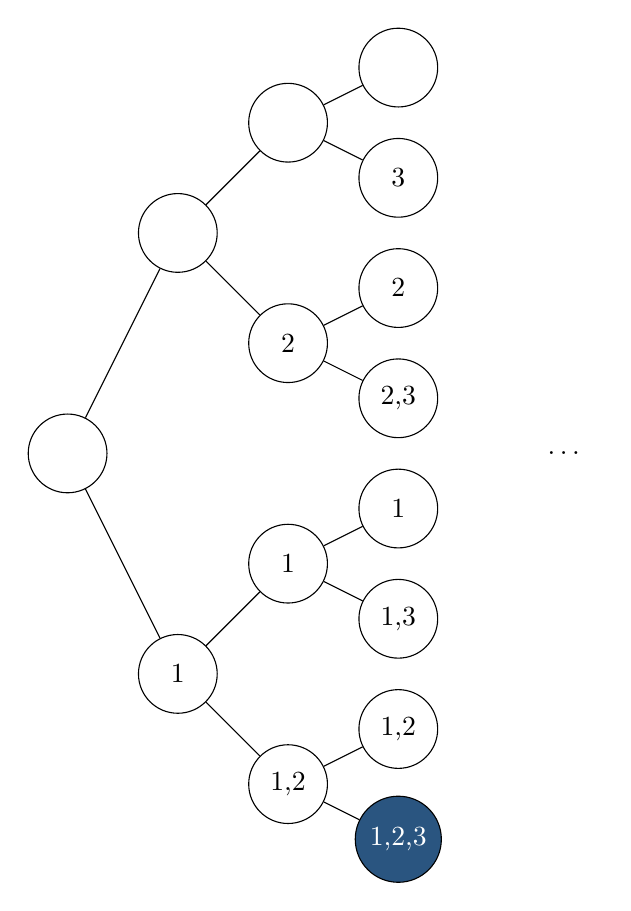
\begin{tikzpicture}[every node/.style={draw,circle, minimum size=1cm}, scale=0.7]
    \node at (0, 7)     (R)         {\(\varnothing\)};

    \node at (2, 11)    (RO)        {\(\varnothing\)};
    \node at (2, 3)     (RA)        {1};

    \node at (4, 13)    (ROO)       {\(\varnothing\)};
    \node at (4, 9)     (ROB)       {2};
    \node at (4, 5)     (RAO)       {1};
    \node at (4, 1)     (RAB)       {1,2};
    
    \node at (6, 14)    (ROOO)      {\(\varnothing\)};
    \node at (6, 12)    (ROOC)      {3};
    \node at (6, 10)    (ROBO)      {2};
    \node at (6, 8)     (ROBC)      {2,3};
    \node at (6, 6)     (RAOO)      {1};
    \node at (6, 4)     (RAOC)      {1,3};
    \node at (6, 2)     (RABO)      {1,2};
    
    % Hervorgehobener Node
    \node[fill={rgb:red,1;green,2;blue,3}] at (6, 0) (RABC) 
        {\textcolor{white}{1,2,3}};
    
    \draw [-] (R) edge (RO) edge (RA);
    \draw [-] (RO) edge (ROO) edge (ROB) (RA) edge (RAB) edge (RAO);
    \draw [-] (ROO) edge (ROOO) edge (ROOC) (ROB) edge (ROBO) edge (ROBC);
    \draw [-] (RAO) edge (RAOO) edge (RAOC) (RAB) edge (RABO) edge (RABC);

    \node[draw=none] at (9, 7) (C) {\(\ldots\)};
\end{tikzpicture}

    \caption{Auswahl der Streckenkombinationen}
    \label{abb:streckrek}
\end{wrapfigure}
Um für jede mögliche Streckenkombination das Vorhandensein eines Dreiecks prüfen zu können, müssen alle möglichen Kombination zunächst einmal aufgestellt werden. Dies habe ich mithilfe einer rekursiven Funktion implementiert.

Ich habe den Streckenauswahlprozess als einen binären Baum interpretiert. Jede Strecke kann entweder Teil einer Auswahl sein -- oder eben auch nicht.

Die Auswahlfunktion wird zunächst mit einer leeren Menge als Auswahl aufgerufen.
Diese leere Menge bildet die Wurzel des Baumes.

Durch Auswahl oder Nicht-Auswahl der ersten Strecke ergeben sich zwei Mengen: Wieder eine
leere Menge (die erste Strecke wurde nicht ausgewählt) oder eine Menge mit der ersten
Strecke als Inhalt (die erste Strecke wurde ausgewählt).

In der nächsten Rekursionsstufe werden dann beide Mengen kopiert und den Kopien jeweils
die zweite Strecke hinzugefügt. Die Mengen nach den ersten drei Rekursionen habe ich
in Abbildung \ref{abb:streckrek} dargestellt.

Sobald eine Menge drei Strecken enthält, kann überprüft werden, ob die enthaltenen
Strecken ein Dreieck bilden.
Hierzu kann Definition \ref{theo:dreiecke} herangezogen werden.

Wenn die Streckenauswahl ein Dreieck bildet, werden die Strecken in einem Vektor
gespeichert und an die nächsthöhere Rekursionsebene zurückgegeben.
Diese gibt dann wiederum einen Vektor über alle Dreiecksvektoren an die nächste Ebene
zurück.
Schlussendlich wird eine Liste über alle möglichen Dreiecke zurückgegeben.

\subsection{Streckenauswahlevaluation}
Zunächst müssen die Schnittpunkte zwischen den Strecken ermittelt werden.
Je nachdem, welchen Funktionstyp die Strecken haben,
müssen verschiedene Verfahren angewandt werden.

Zwischen zwei linearen Funktion lässt sich der Schnittpunkt folgendermaßen durch
Gleichsetzen ermitteln:

\begin{equation}
    \begin{aligned}
        m_1x+n_1 &= m_2x+n_2             &&\quad\vert -n_2          \\
        m_1x+n_1-n_2 &= m_2x             &&\quad\vert -m_1x         \\
        n_1-n_2 &= (m_2-m_1)x            &&\quad\vert \div(m_2-m_1) \\
        x &= \frac{n_1-n_2}{m_2-m_1}                                \\
        y &= m_1x+n_2                                               \\
    \end{aligned}
    \label{eq:linearschnitt}
\end{equation}

Der Schnittpunkt zwischen einer Geraden \(y=m_1x+n_1\) und einer Senkrechten \(x=n_2\),
liegt bei der y-Koordinate, die die Gerade an der x-Stelle der Senkrechten annimmt.
Zur Ermittlung dieses Wert muss die Senkrechte in die Gerade eingesetzt werden:

\begin{equation}
    \begin{aligned}
        x &= n_2                    \\
        y &= m_1 \times x + n_1 \qquad\vert\ \text{einsetzen}  \\
        y &= m_1 \times n_2 + n_1   \\
    \end{aligned}
    \label{eq:senkrechtschnitt}
\end{equation}

Falls beide Funktionen Senkrechten sind, können sie sich nur schneiden,
wenn Start- oder Endpunkte sich überlappen.
Schließlich sind aufeinander liegende Strecken laut Aufgabenstellung ausgeschlossen.
Wenn Start- und Endpunkt zweier Senkrechten sich überlappen,
können diese beiden Senkrechten unmöglich gemeinsam mit einer Geraden
ein Dreieck bilden. Daher kann angenommen werden, dass eine Auswahl mit zwei Senkrechten
kein Dreieck bilden kann.

\begin{wrapfigure}{r}{0.3\textwidth}
    \begin{center}
    \begin{tikzpicture}
    \draw (3,1) -- (1,1);
    \draw (2,2) -- (0,0);
    \draw (1,3) -- (1,1);
    
    \fill[red] (1,1) circle (.1cm);
\end{tikzpicture}

    \end{center}
    \caption{Dreieck mit der Flächengröße 0}
    \label{abb:dreieck}
\end{wrapfigure}
Abschließend muss für jeden Schnittpunkt geprüft werden,
ob er zwischen dem Start- und Endpunkt beider Strecken liegt.
Schließlich können die Geraden sich außerhalb der Strecken,
die nur ein Abschnitt der Geraden sind, schneiden.
Im Sinne der Aufgabenstellung zählen nur Schnittpunkte der Strecken.

Außerdem muss überprüft werden, dass die Schnittpunkte sich nicht gleichen.
Schließlich hätte das Dreieck sonst einen Flächeninhalt von Null.
Ein Beispiel für sich gleichende Schnittpunkte ist Abb. \ref{abb:dreieck}.

Obengenannte Rechnungen sind in der Geradenklasse \texttt{line} in der Funktion
\texttt{calculateIntersections} implementiert.
Je nachdem, welche Strecken der Funktion übergeben wurden,
führt sie die entsprechenden Rechnungen durch.
Die Funktion gibt ein \texttt{pair<bool, Coord>} zurück.
Wenn der Bool auf true steht,
ist im zweiten Feld des Paars ein Schnittpunkt vermerkt.
Ansonsten wurde kein Schnittpunkt gefunden.

In einer weiteren Funktion, \texttt{isOnLine(..)}, wird, sodenn
die Geraden sich schneiden, überprüft, ob die übergebene Koordinate zwischen
oder auf den die Strecke begrenzenden Punkten liegt.

Wenn alle Strecken sich wie oben beschrieben schneiden und die Schnittpunkte verschieden
sind, bilden die übergebenen Strecken ein Dreieck.

\subsection {Grafische Ausgabe}
Die grafische Ausgabe wurde mit HTML realisiert. Seit HTML5 kann SVG inline genutzt
werden.
Dies macht sich mein Programm zu nutze, indem es die Zeichnung und das Dreieck
als SVG-Objekte im HTML-Dokument ausgibt.
Den Ausgabecode habe ich aus Platzgründen nicht im Dokument aufgeführt.
